\documentclass{article}
\usepackage[utf8]{inputenc}
\usepackage[french]{babel}
\usepackage{graphicx}
\usepackage[left=2.8cm,right=2.8cm,top=2.5cm,bottom=2.5cm]{geometry}
\usepackage[normalem]{ ulem }
\usepackage{soul}

\title{Rapport 1 : La modélisation de données}

\author{Guilmot Gautier \\ Hansart Charlotte \\ Lardinois Maxence \\ Mulders Zélie \\ Tihon Simon \\ Groupe E }

\date{February 2015}

\begin{document}

\maketitle

\section{Introduction}
Afin de réaliser notre schéma conceputel ORM, nous avons tout d'abord dû établir des faits élémentaires. Pour cela nous nous sommes basés sur des captures d'écran du prototype de l'application, ainsi que sur d'autres documents fournis ou trouvés sur le web. Ensuite nous avons transformé notre schéma ORM en une base de données relationnelle que nous avons remplie avec quelques données représentatives. Pour finir, nous avons fait quelques requêtes intéressantes pour vérifier l'intégrité de notre base de données.

\section{Faits élémentaires}
\begin{itemize}\renewcommand{\labelitemi}{$\bullet$}
\item Une boisson se vend à un prix de vente 
\item Une boisson coûte un prix d'achat
\item Une boisson a un stock
\item Une boisson est d'un certain type
\item Une boisson est décrite par une description
\item Une boisson est décrite par une image
\item Une boisson a un seuil minimal 
\item Une boisson a un stock maximum
\item Une commande contient une boisson en une certaine quantité
\item Une commande est gérée par un serveur
\item Une commande est rattachée à une table
\item Une commande a une date
\item Une commande est passée par un client
\item Un client a un mot de passe
\item Un client est représenté par un avatar
\item Un client s'exprime en une langue
\item Un client a un sexe
\item Un serveur est représenté par une photo
\item Un serveur possède un mot de passe
\item Un serveur a un sexe 
\item Un serveur remplit un statut (Gérant ou non)
\item Un serveur a un numéro de téléphone
\item Un serveur a un numéro de compte bancaire
\item Un serveur porte un prénom
\item Un serveur porte un nom


\end{itemize}

\section{Schéma conceptuel ORM}
\vspace{-0.2cm}
\hspace{-2cm}
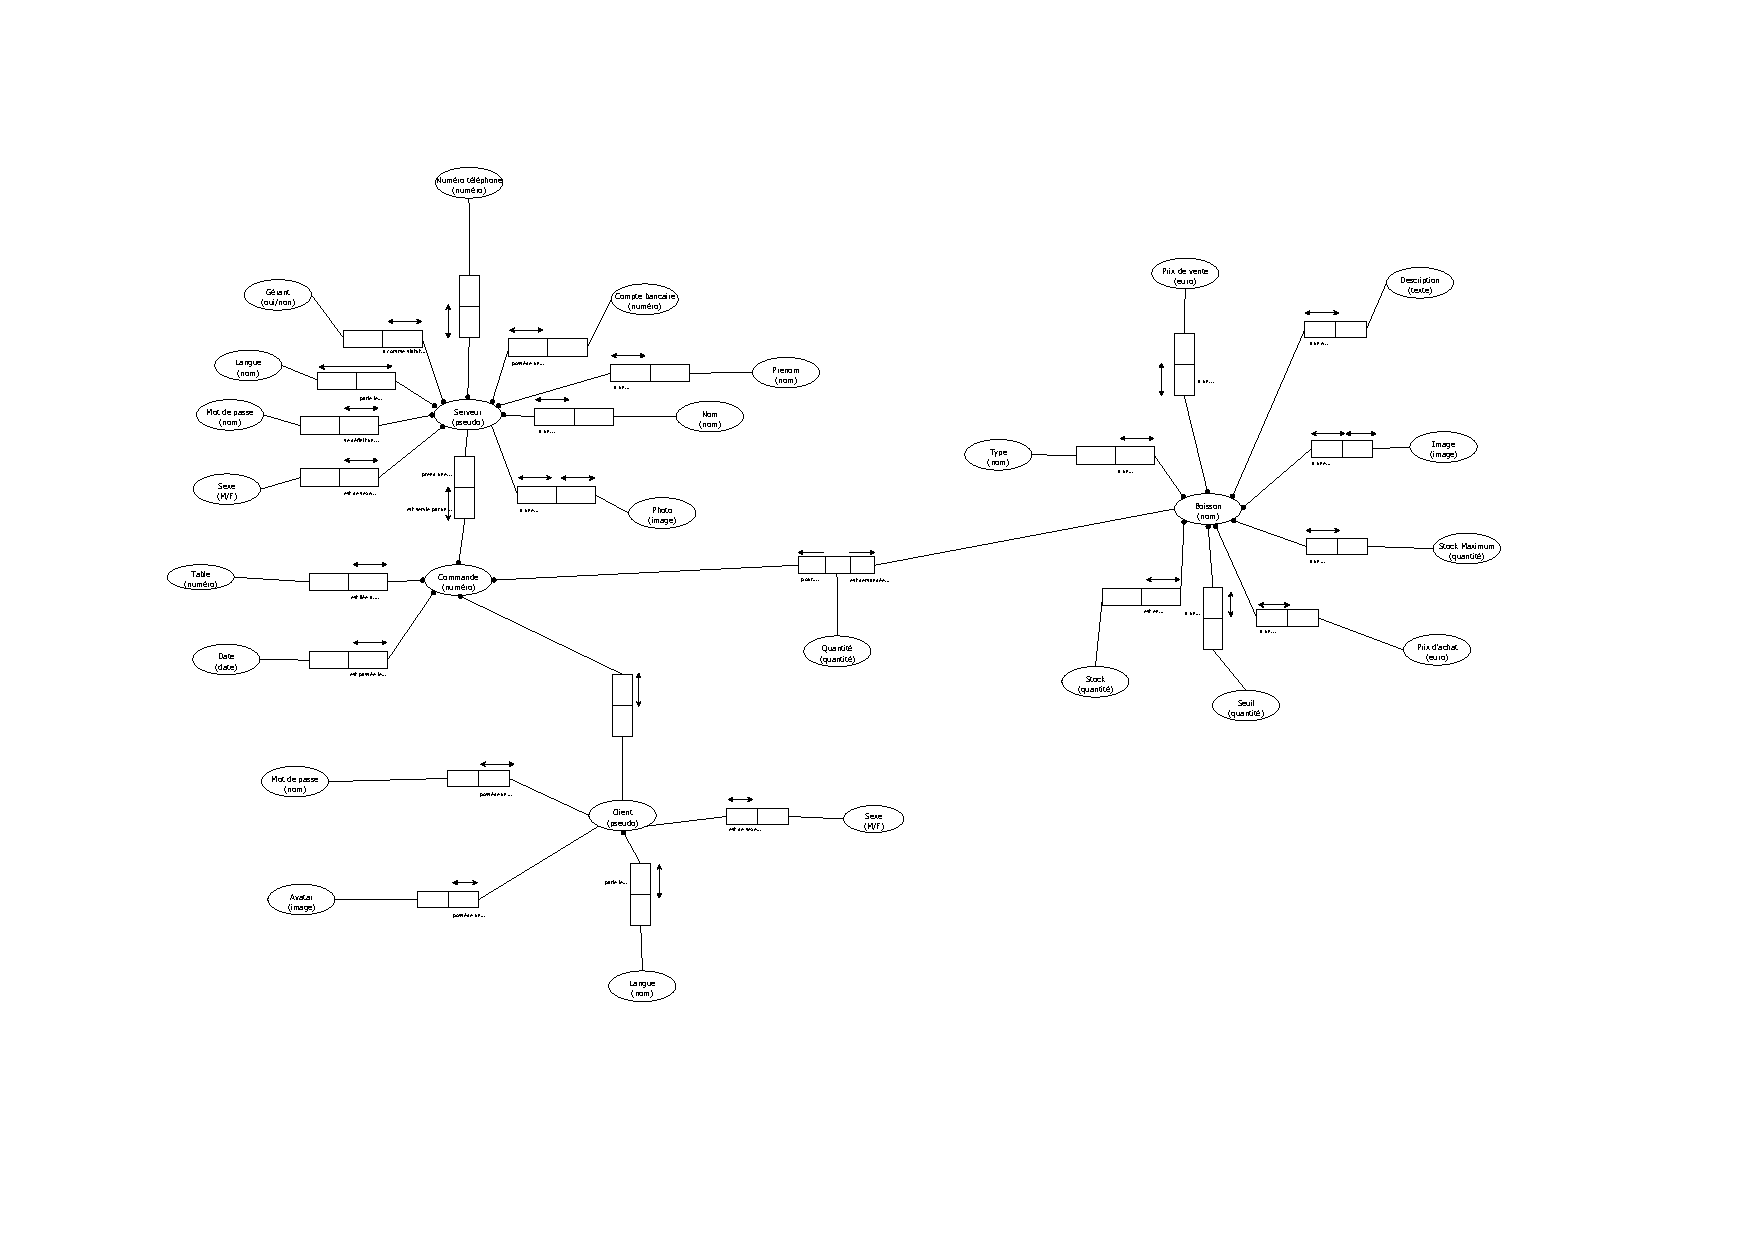
\includegraphics[scale=1, angle=90, trim=3 20 115 3, clip=true]{img/ORM_final.pdf}

\section{Schéma relationnel}
\textbf{Boisson(\uuline{NomBoisson}, PrixVente, Stock, Max, Seuil, Description, Type, Image)}

\textbf{Client(\uuline{PseudoC}, Langue, [Mdp], [Sex\{M,F\}], [Avatar])}

\textbf{Commande(\uuline{NumCommande}, Date, PseudoS, PseudoC, NTable)}

\textbf{Detail(\uuline{NumeroD}, Quantite, NomBoisson, NumCommande)}

\textbf{Serveur(\ul{PseudoS, Mdp}, Sex\{M,F\}, Langue, Gerant\{Oui,Non\}, Ntel, CptBanq, Prenom, Nom, [Photo])} 

\section{SQLite et Requêtes SQL}
Voir fichier zip

\section{Choix de conception}
\subsection{Général}
Afin d'offrir à l'utilisateur un confort d'utilisation maximum, nous avons fait plusieurs choix de conception. Ils portent principalement sur les "objets de base" nécessaires au bon fonctionnement d'un bar : Clients, Boissons, Serveurs.

Tout d'abord s'est posée à nous la question des clients. Si un client n'est pas enregistré, ne peut-il donc pas commander ? A cet effet, nous avons pensé à faire un compte "default", sans mot de passe, pour tout client désireux de commander via l'application sans forcément devoir passer par un enregistrement.

Ensuite, au niveau des serveurs, nous avons pensé à enregistrer toutes les langues connues ; ce afin de pouvoir associer à un client qui passe une commance un serveur parlant, ou sachant parler, la même langue que lui. Ainsi, les clients se sentiront mieux accueillis et ressortiront plus satisfaits de leur expérience dans le bar.

Puis nous nous sommes intéressés à des détails : possibilité d'avoir un avatar pour un client, obligation pour un serveur d'avoir une photo, interdiction d'utiliser la même image pour deux boissons différentes, et autres, visibles sur le schéma ORM.

\subsection{Extensions}
En plus du programme de base, notre groupe a voulu installer deux extensions.
La première consiste en la possibilité de faire aisément des statistiques, portant par exemple sur le profit net du bar en une journée, la bière la plus vendue sur une durée déterminée, le client le plus buveur, le serveur le plus efficace et vendeur, et d'autres encore. Nous avons dû rajouter le prix d'achat des produits dans notre base de donnée pour permettre plus de statistiques.

La deuxième extension porte sur la gérance de la base de donnée. Un serveur pourra ou non être gérant, c'est-à-dire qu'il pourra ou non modifier les stocks (achats, gaspillages, autres), rajouter de nouvelles boissons à la liste, modifier la liste de serveurs (engagement, retraite, etc), et tout ce dont a besoin un patron pour faire tourner correctement son bar.

\section{Conclusion}
Notre application aidera donc à la gestion du bar, des commandes, clients et serveurs, de manière simple et intuitive, et permettra même d'obtenir certaines statistiques utiles à cet effet. Gérer un bar n'aura jamais été aussi simple.


"Bartender, soyez servis à l'heure !"

\end{document}
